\documentclass[10pt]{article}
\newcounter{myCounter}
\newcommand{\head}[1]{\textbf{#1}}
\newcommand{\keyword}[2][\bfseries]{{#1#2}}
\usepackage{CJK}%preamble part
\usepackage{graphicx}
\usepackage{sidecap}
\usepackage[a4paper, inner=1.5cm, outer=3cm, top=2cm, bottom=3cm, bindingoffset=1cm]{geometry}
\usepackage{epstopdf}
\usepackage{array}
\setlength{\extrarowheight}{4pt}
\begin{document}


\begin{CJK}{GBK}{song}
\title{显式Runge Kutta 法绝对稳定区域作图练习} % This is the title
\author{数33 赵丰 2013012178}
\date{Auguest 26,2016}
\maketitle
%\section{Abstract}
%\section{introduction}
\section{Presentation}
\setlength{\parindent}{2em}
用显式Runge Kutta 法求解试验方程:
$$ y'=\lambda y(0)=y_0;$$
可得到迭代公式为:
$$ y_{n+1}=E(z)y_n$$
其中$z=h\lambda$而对应于s阶显式Rugge Kutta 法,$E(z)$为$e^z$的前s阶Taylor 展开。\\
\begin{tabular}{cl}
\hline
\textbf{阶数s} & \textbf{稳定区域边界表达式} \\
\hline
1 & $ |1+z|=1$ \\
2 & $ |1+z+z^2|=1$ \\
3 & $ |1+z+\frac{z^2}{2}+\frac{z^3}{6}|=1$ \\
4 & $ |1+z+\frac{z^2}{2}+\frac{z^3}{6}+\frac{z^4}{24}|=1$ \\
\hline
\end{tabular}
\begin{figure}[!h]
\caption{
\parbox[l]{5cm}{
利用Matlab的Contour Plot 可以作出
s=1,2,3,4对应的稳定区域的边界曲线 
}}
\centering
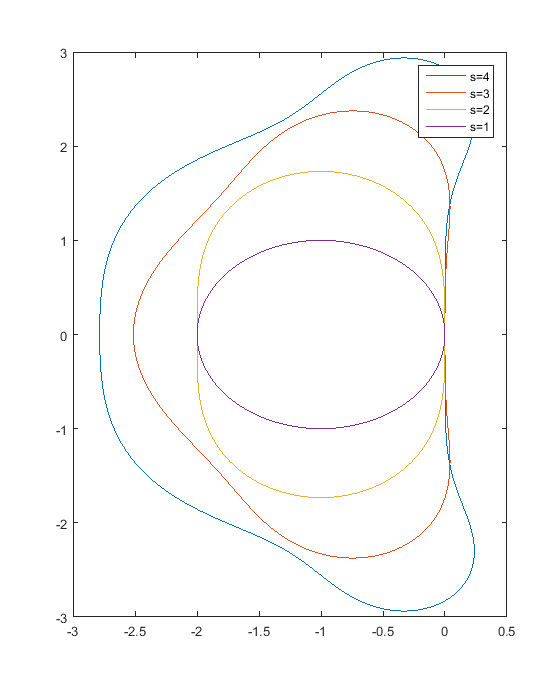
\includegraphics[width=7cm]{RungeKuttaAs.png}
\end{figure}

由上图可见,阶数越高,绝对稳定区域越大。
\end{CJK}
\end{document}